\chapter{Subdivison Tools und Bibliotheken}

Im Bereich Subdivison Algorithmen gibt es schon viele mächtige Bibliotheken und Datenstrukturen.
Für das Team-Projekt bietet es sich an, diese zu evaluieren und passende Basisfunktionen wiederzuverwenden.
Dieses Kapitel vergleicht die gängigen C++-Bibliotheken und Datenstrukturen.
Gesucht wird eine einfache Datenstruktur, um polygonale Netze verarbeiten zu können.
Im Allgemeinen besteht solch eine Datenstruktur aus Ecken (Verteices), Kanten (Edges) und Flächen (Faces).
Zusätzlich muss noch die Beziehung zwischen den Objekten hinterlegt werden.


\section{OpenMesh}

OpenMesh wird von der \acs{RWTH} Aachen entwickelt und stellt eine mächtige Datenstruktur für polygonale Netze bereit.
Es steht unter der \acs{LGPL} v3 Lizenz ("with exception") und kann für unseren Fall somit problemlos verwendet werden.

\subsection{Datenstrukturen und Algorithmen}

OpenMesh implementiert eine Datenstruktur für polygonale Meshes. Darüber hinaus sind sogar bereits einige Subdivision Algorithmen implementiert, die auf der OpenMesh Datenstruktur arbeiten können. Zum Funktionsumfang gehören folgende Algorithmen.
\begin{enumerate}
\item Uniform subdivision
\begin{itemize}
	\item Loop
	\item SQRT3
	\item Modified Butterfly
	\item Interpolationg SQRT3 LG
	\item Composite
	\item Catmull Clark
\end{itemize}
\item Adaptive subdivision
\begin{itemize}
	\item Adaptive Composite
\end{itemize}
\item Simple subdivision
\begin{itemize}
	\item Longest Edge
\end{itemize}
\end{enumerate}

OpenMesh implementiert eine \emph{halfedge} Datenstruktur.
Diese \emph{edge-based} Datenstrukturen speichern die Information über die Verbindungen zwischen Eckpunkten (Vertices) in den Kanten (Edges), während
\emph{face-based} Datenstrukturen die Verbindungsinformation zwischen den Eckpunkten und Nachbarn in den Flächen (Face) speichern.\\
Jede Kante (Edge) referenziert also folgende Objekte:
\begin{itemize}
	\item 2 Eckpunkte (Vertices)
	\item eine Fläche (Face)
	\item die nächsten zwei Kanten (Edges) der Fläche
\end{itemize}

Halfedge bedeutet nun, dass eine Kante in 2 Halbkanten (Halfedge) aufgeteilt wird. Jede Halbkante hat nur eine Richtung.
Zwei Ecken A und B sind nun also über 2 Halbkanten (1. Halkante von A nach B und 2. Halbkante con B nach A) miteinander verbunden.
Dies bringt den Vorteil, dass man über die Kanten einer Fläche sehr einfach iterieren kann, man muss dazu lediglich den Halbkanten folgen.

\subsection{OpenFlipper}

Aufbauend auf OpenMesh wurde von der \acs{RWTH} Aachen zusätzlich das flexible pluginbasierte Framework OpenFlipper enwickelt.
Damit können geometrische Objekte modelliert und verarbeitet werden. Intern wird auf die Datenstrukur OpenMesh zurückgegriffen.
Für die grafische Oberfläche wird QT verwendet.
Mit OpenFlipper kann man über die Oberfläche Netze erstellen und über die Oberfläche die in OpenMesh implementierten Subdivision Algorithmen anwenden.
Abbildung~\ref{fig:openflipper} zeigt die Benutzeroberfläche von OpenFlipper
\begin{figure}[h]
  \caption{OpenFlipper}
  \centering
  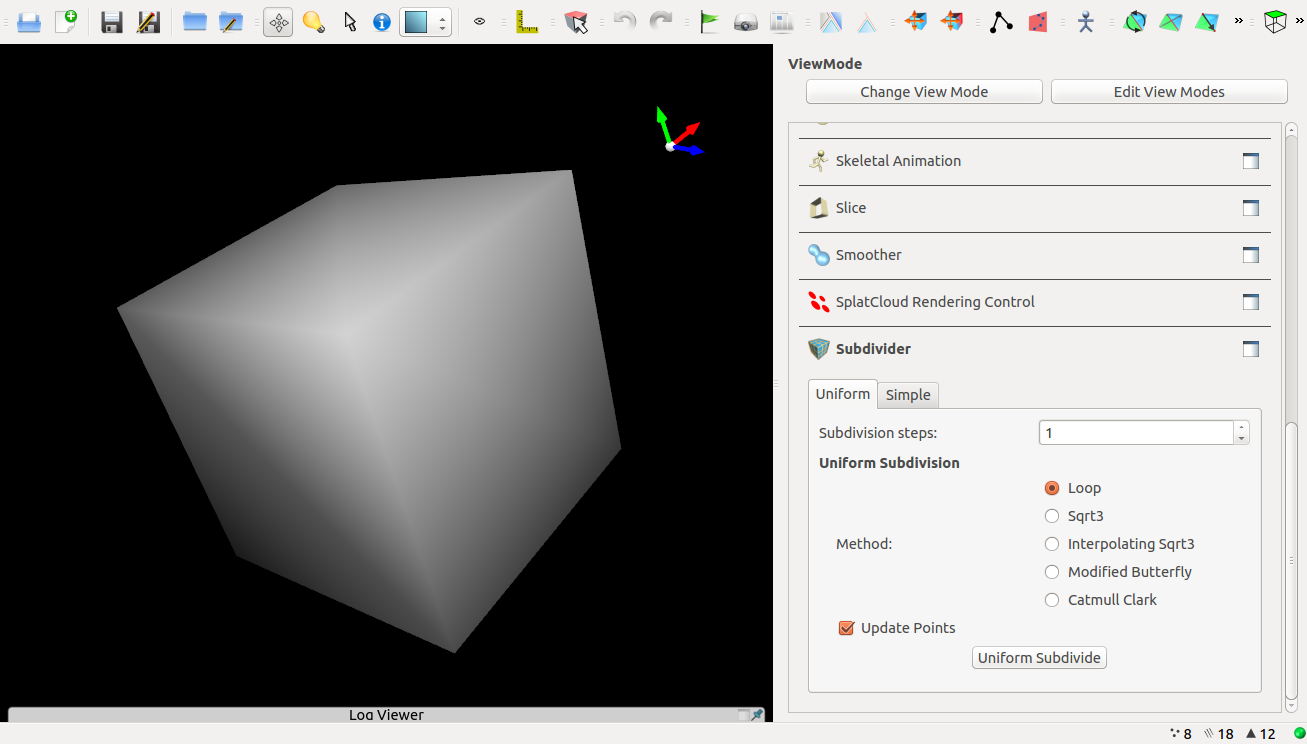
\includegraphics[width=0.8\textwidth]{content/media/openflipper_cube}
  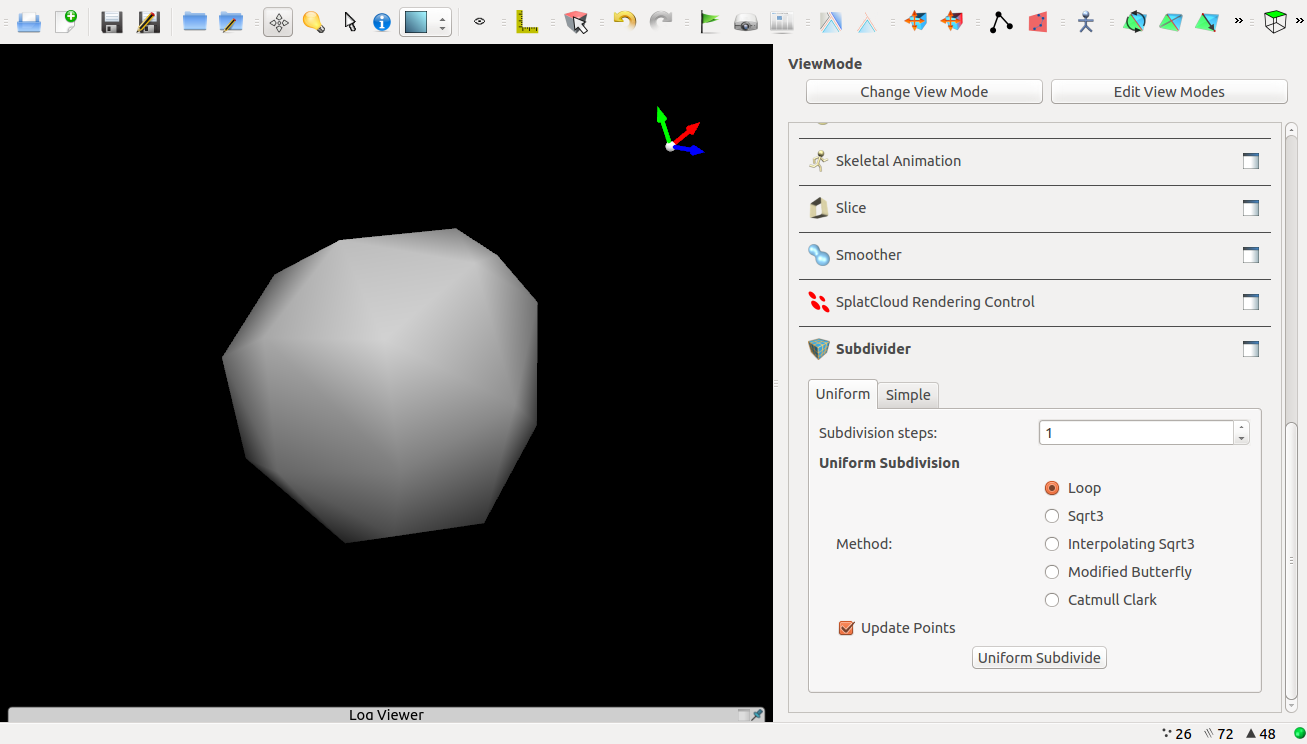
\includegraphics[width=0.8\textwidth]{content/media/openflipper_loop}
  \label{fig:openflipper}
\end{figure}


\section{Surface Mesh}

Surface Mesh ist eine einfache und effizente Datenstruktur um polygonale Netze beschreiben zu können.
Die Datenstruktur wurde alse einfachere Alternative zu OpenMesh von der Bielefeld Graphics \& Geometry Group entwickelt.
Die Datenstruktur soll vergleichsweise einfacher zu benutzen sein und eine bessere Performance und einen geringeren Speicherverbrauch mitbringen.
Analog zu OpenMesh implementiert Surface Mesh eine halfedge Datenstruktur.
Die Verbindungsinformation der Kanten werden also in einem Paar aus zwei gerichteten Halbkanten gespeichert.
Abbildung~\ref{fig:sm_halfedge} visualisiert den Zusammenhang der Halbkanten und Ecken.

\begin{figure}[h]
  \caption{Surface Mesh - Halfedge Verbindungen}
  \centering
  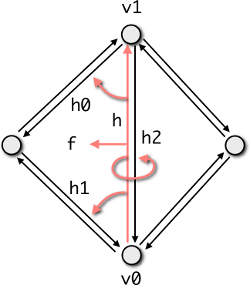
\includegraphics[width=0.3\textwidth]{content/media/sm_connectivity-queries}
  \label{fig:sm_halfedge}
\end{figure}

Da Surface Mesh auch als Halfedge Datenstruktur implementiert ist, kann ähnlich effizient zu OpenMesh über die Kanten iteriert werden.
Listing~\ref{lst:sm_iterate} zeigt einige Basisoperiation, die möglich sind.
Die Variablen sind in Abbildung~\ref{fig:sm_halfedge} gleich benannt. \cite{OpenGP.24.07.2015}

\begin{lstlisting}[style=myCppStyle, caption=Surface Mesh - Iterieren über Kanten einer Fläche, label=lst:sm_iterate]
Surface_mesh::Halfedge h;
Surface_mesh::Halfedge h0 = mesh.next_halfedge_handle(h);
Surface_mesh::Halfedge h1 = mesh.prev_halfedge_handle(h);
Surface_mesh::Halfedge h2 = mesh.opposite_halfedge_handle(h);
Surface_mesh::Face     f  = mesh.face_handle(h);
Surface_mesh::Vertex   v0 = mesh.from_vertex_handle(h);
Surface_mesh::Vertex   v1 = mesh.to_vertex_handle(h);
\end{lstlisting}

Um das Netz zu verändern oder zu editieren unterstützt die Datenstruktur high-level Operationen um die Topology zu verändern.
Die Datenstuktur kann mit \emph{Edge Collapse}, \emph{Edge Split} und \emph{Edge Flip} das Netz ändern.
Die Operationen sind in Abbildung~\ref{fig:sm_topology} dargestellt. \cite{OpenGP.24.07.2015}

\begin{figure}[h]
  \caption{Surface Mesh - High-level Operationen zum Ändern der Topology}
  \centering
  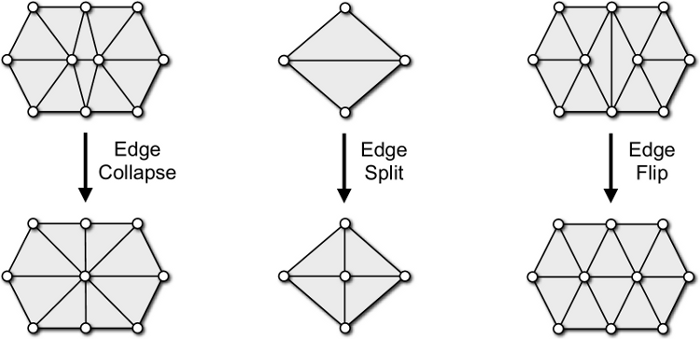
\includegraphics[width=0.8\textwidth]{content/media/sm_topology-changes}
  \label{fig:sm_topology}
\end{figure}

\section{OpenSubdiv}

OpenSubdiv wird von Pixar entwickelt und ist eine mächtige Bibliothek, die Subdivision Algorithmen und Datenstrukturen implementiert.
Die Bibliothek ist optimiert auf Performance und unterstützt paralleles Rechnen auf CPU und GPU.
Primär wird die Bibliothek von Pixar zum erstellen von animierten Filmen verwendet.
OpenSubdiv ist lizensiert unter der Apache License und darf somit frei für kommerzielle und nicht kommerzielle Nutzung.

\begin{figure}[h]
  \caption{Pixar OpenSubdiv Architektur}
  \centering
  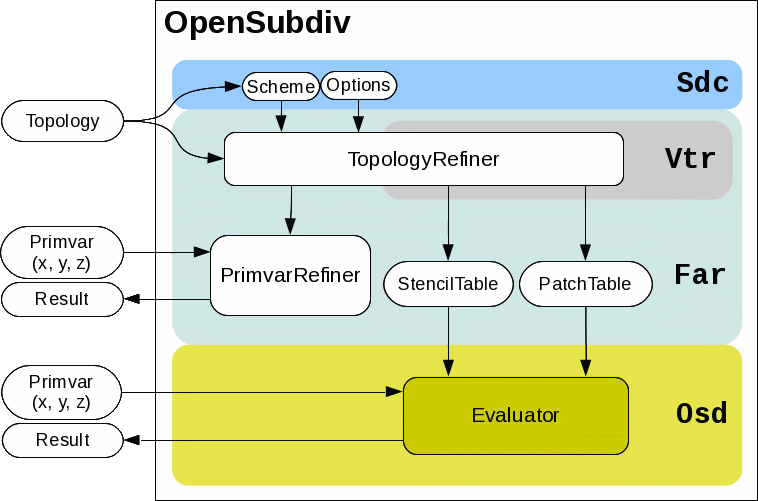
\includegraphics[width=0.9\textwidth]{content/media/pixar_opensubdiv}
  \\Quelle: \cite{Pixar.27.07.2015}
  \label{fig:pixar_opensubdiv}
\end{figure}

Abbildung~\ref{fig:pixar_opensubdiv} zeigt einen Überblick über die OpenSubdiv Bibliothek.
Die Bibliothek besteht insgesamt aus den 4 Schichten \ac{Sdc}, \ac{Vtr}, \ac{Far} und \ac{Osd}.
\cite{Pixar.27.07.2015}

\begin{description}
 \item[\acs{Sdc}] ist der unterste Layer in der Architektur und implementiert die konkreten Subdivision Details.
 Dazu gehören Typen, Optionen und Eigenschaften für die konkreten Subdivision Algorithmen.
 \item[\acs{Vtr}] beinhaltet Klassen, die das Netz für effiziente Verfeinerung in einer Zwischenrepresentation darstellen.
 Diese Schicht ist nur für den internen Gebrauch gedacht.
 \item[\acs{Far}] ist die zentrale Schnittstelle um Netze mit Subdivision Algorithmen zu verarbeiten.
 \item[\acs{Osd}] beinhaltet geräteabhängigen Code, um Objekte aus der Schicht \acs{Far} auch in unterschiedlichen Backends wie
 \acs{CUDA} oder OpenCL ausführbar zu machen.
\end{description}

Von OpenSubdiv werden die Subdivision Algorithmen \emph{Catmull-Clar}, \emph{Loop} und \emph{Bilinear} unterstützt. \cite{Pixar.27.07.2015}

\section{CGoGN}

// TODO
\cite{ieee:wpan}

\section{\acf{CGAL}}

// TODO


\section{Sonstige Tools}


\subsection{BViewer}

